% \iffalse meta-comment ---------------------------------------------
% Copyright (C) 2021 SJTUG
%
% Licensed under the Apache License, Version 2.0 (the "License");
% you may not use this file except in compliance with the License.
% You may obtain a copy of the License at
%
%     http://www.apache.org/licenses/LICENSE-2.0
%
% Unless required by applicable law or agreed to in writing, software 
% distributed under the License is distributed on an "AS IS" BASIS,
% WITHOUT WARRANTIES OR CONDITIONS OF ANY KIND, either express or implied.
% See the License for the specific language governing permissions and
% limitations under the License.
%
% ------------------------------------------------------------------- \fi
% \iffalse
%<*package>
\NeedsTeXFormat{LaTeX2e}
\ProvidesPackage{beamerthemesjtubeamermin}[2021-08-14 sjtubeamermin parent theme v1.0]
%</package>
% \fi
% \CheckSum{0}
% \StopEventually{}
% \iffalse
%<*root>
% ------------------------------------------------------------------- \fi
% Entry Point. The root style.
%    \begin{macrocode}
\RequirePackage{kvoptions}
\RequirePackage{iftex}

\SetupKeyvalOptions{
  family=sjtubeamer,
  prefix=sjtubeamer@
}

\DeclareBoolOption{maxplus}
\DeclareBoolOption{max}
\DeclareBoolOption{min}
\sjtubeamer@maxplustrue

\DeclareBoolOption{red}
\DeclareBoolOption{blue}
\sjtubeamer@redtrue

\DeclareBoolOption{bannertitle}

\ProcessKeyvalOptions{sjtubeamer}

\ifsjtubeamer@bannertitle
  \sjtubeamer@DisableOption{warning}{bannertitle}
  \sjtubeamer@maxplustrue
\fi

\ifsjtubeamer@min
  \ifsjtubeamer@red
    \PassOptionsToPackage{color=red}{sjtubeamermin}
  \else
    \PassOptionsToPackage{color=blue}{sjtubeamermin}
  \fi
  \usetheme{sjtubeamermin}
\else
  \ifsjtubeamer@red
    \PassOptionsToPackage{red}{sjtubeamermax}
  \else
    \PassOptionsToPackage{blue}{sjtubeamermax}
  \fi
  \ifsjtubeamer@maxplus
    \PassOptionsToPackage{bannertitle}{sjtubeamermax}
  \fi
  \usetheme{sjtubeamermax}
\fi
%    \end{macrocode}
%
% \iffalse
%</root>
% ------------------------------------------------------------------- \fi
% \iffalse
%<*max>
% ------------------------------------------------------------------- \fi
% A temporary move for max option.
%    \begin{macrocode}

\RequirePackage{biblatex}

\SetupKeyvalOptions{
  family=sjtubeamermax,
  prefix=sjtubeamermax@
}
\DeclareBoolOption{bannertitle}
\DeclareBoolOption{red}
\DeclareBoolOption{blue}
\sjtubeamermax@redtrue
\sjtubeamermax@bannertitletrue
\ProcessKeyvalOptions{sjtubeamermax}

\usetheme{Szeged}
\usecolortheme{dolphin}

\usefonttheme{structurebold}
\useinnertheme{circles}
\setbeamertemplate{blocks}[rounded]

\ifsjtubeamermax@red
  \definecolor{SJTUPrimary}{RGB}{200,22,30}
\fi

\ifsjtubeamermax@blue
  \definecolor{SJTUPrimary}{RGB}{0,64,152}
\fi

\setbeamercolor{structure}{fg=SJTUPrimary}
\setbeamertemplate{background}{
\includegraphics[width=\paperwidth]{vi/sjtu-miao.png}}

\ifsjtubeamermax@red
  \logo{
\includegraphics[height=1.5cm]{vi/sjtu-vi-badge-red.pdf}}
  \setbeamercolor{banner title page}{fg=SJTUPrimary,bg=white}
\fi

\ifsjtubeamermax@blue
  \logo{
\includegraphics[height=1.5cm]{vi/sjtu-vi-badge-blue.pdf}}
  \setbeamercolor{banner title page}{fg=white,bg=SJTUPrimary}
\fi

\ifsjtubeamermax@bannertitle
  \defbeamertemplate*{title page}{sjtured}[1][]
  {
    \nointerlineskip%
    \begin{beamercolorbox}[wd=\paperwidth, ht=\paperheight]{empty}
      \usebeamercolor{banner title page}% 
      \begin{tikzpicture}
        \pgfmathsetlengthmacro{\outslant}{\the\paperwidth - 0.8cm}
        \node[anchor=north west, inner sep=0, outer sep=0] at (0,\the\paperheight){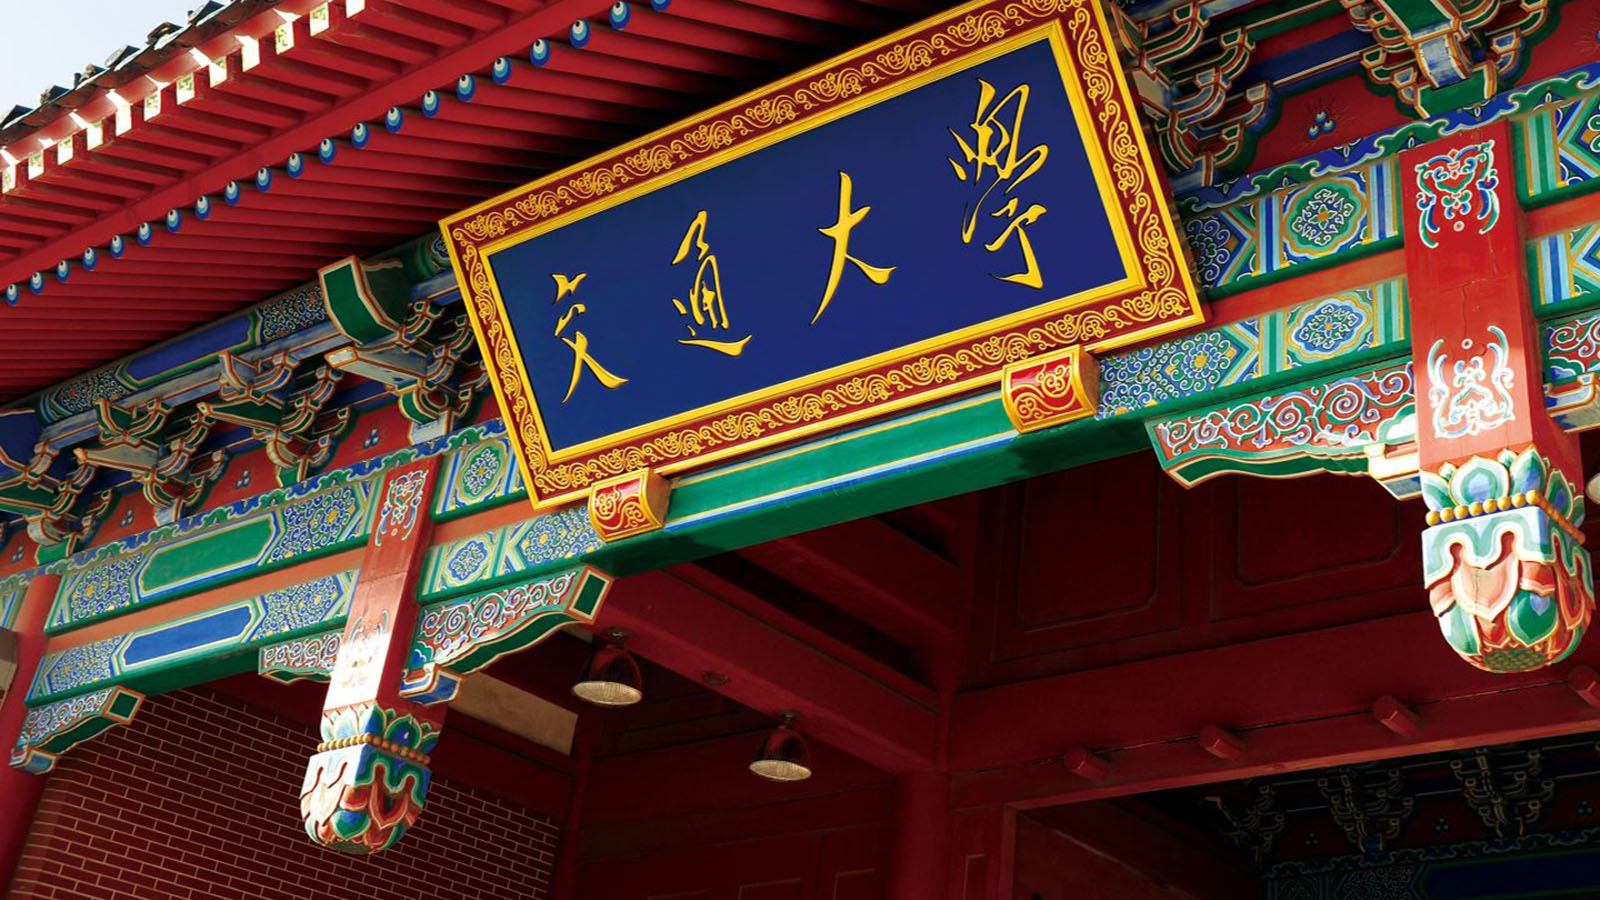
\includegraphics[height=\paperheight]{vi/title-background.jpg}};
        \fill[color=white] (0,0) rectangle(\the\paperwidth,3.9);
        \fill[color=bg]  (0,0) rectangle(\the\paperwidth,3.88);
        \node[anchor=north west, text width=.8\paperwidth, fg] at (0.8,3.6){%
        \ifx\insertsubtitle\@empty%
          {\huge\bfseries\inserttitle}\\
          \else%
          {\Large\bfseries\inserttitle}\\
          {\small\insertsubtitle}\\
        \fi%
        };
        \node[anchor=south west, text width=.8\paperwidth, fg] at (0.8,0.45){%
        {\small\insertauthor}\\
        {\small\insertinstitute}\\
        {\small\insertdate}%
        };
        \node[anchor=south east, inner sep=0, outer sep=0] at (\outslant,0.5){
          \ifsjtubeamermax@red
            
\includegraphics[height=1cm]{vi/sjtu-vi-logo-red.pdf}
          \fi

          \ifsjtubeamermax@blue
            
\includegraphics[height=1cm]{vi/sjtu-vi-logo-white.pdf}
          \fi
        };
      \end{tikzpicture}
    \end{beamercolorbox}
  }
\fi
%    \end{macrocode}
% \iffalse
%</max>
% ------------------------------------------------------------------- \fi

% \iffalse
%<*min>
% ------------------------------------------------------------------- \fi
%
% \subsection{Parent Theme}
%
% The primary job of this package is to load the component sub-packages of the
% \themename theme and route the theme options accordingly. It also
% provides some custom commands and environments for the user.
%
%   This declares that the following setup is avaliable for all modes.
%    \begin{macrocode}
\mode<all>
%    \end{macrocode}
%
% \subsubsection{Option Declaration}
%
% \begin{macro}{navigation}
%   Change the appearence of the navigation bar, which will affect in the outer theme.
%    \begin{macrocode}
\DeclareOptionBeamer{navigation}{
    \PassOptionsToPackage{navigation=#1}{beamerouterthemesjtubeamermin}
}
%    \end{macrocode}
% \end{macro}
%
% \begin{macro}{lang}
%   Set the language of this beamer. Two options are provided:
%   \begin{description}
%    \item[cn] Chinese. The loaded logo will be the original one. And the package for chinese character support (C\TeX or CJK) will be loaded as well. The bibliography will also get affected.
%    \item[en] English. The loaded logo will be the English one.
%   \end{description}
%   This option will get passed to both inner and outer theme.
%    \begin{macrocode}
\DeclareOptionBeamer{lang}{
    \def\beamer@sjtubeamermin@lang{#1}
    \PassOptionsToPackage{lang=#1}{beamerouterthemesjtubeamermin}
    \PassOptionsToPackage{lang=#1}{beamerinnerthemesjtubeamermin}
}
\def\beamer@sjtubeamermin@langcn{cn}%
\def\beamer@sjtubeamermin@langen{en}%
%    \end{macrocode}
% \end{macro}
%
% 
% \begin{macro}{cjk}
%   Choose to use `CJK' package. If this option is open, the document body should be covered by \verb"\begin{CJK}{UTF8}{hei}" and \verb"\end{CJK}".
%    \begin{macrocode}
\DeclareOptionBeamer{cjk}{\def\beamer@sjtubeamermin@cjk{#1}}
\def\beamer@sjtubeamermin@cjktrue{true}%
\def\beamer@sjtubeamermin@cjkfalse{false}%
%    \end{macrocode}
% \end{macro}
% 
% \begin{macro}{color}
%   Provided two options:
%   \begin{description}
%     \item[blue] The default selection.
%     \item[red] The recomended theme for non-scitific scenario. 
%   \end{description}
%   This option will be passed to the color theme and inner theme.
%    \begin{macrocode}
\DeclareOptionBeamer{color}{
    \PassOptionsToPackage{color=#1}{beamercolorthemesjtubeamermin}
    \PassOptionsToPackage{color=#1}{beamerinnerthemesjtubeamermin}
}
%    \end{macrocode}
% \end{macro}
%
% \begin{macro}{pattern}
%   Provided three options to affect the pattern in the slides:
%   \begin{description}
%     \item[none] No patterns will be generated.
%     \item[title] A pattern array will get generated in the title page.
%     \item[all] Besides the title page, the frame title of section start page will get a stamp array pattern.
%   \end{description}
%   This option will get passed to the outer theme and inner theme.
%    \begin{macrocode}
\DeclareOptionBeamer{pattern}{
    \PassOptionsToPackage{pattern=#1}{beamerouterthemesjtubeamermin}
    \PassOptionsToPackage{pattern=#1}{beamerinnerthemesjtubeamermin}
}
%    \end{macrocode}
% \end{macro}
%
% \begin{macro}{gbt}
%   Choose the behaviour of citing.
%   \begin{description}
%     \item[false] Use \verb"biblatex" to cite.
%     \item[bibtex] Use \verb"bibtex" to cite.
%     \item[true] Use \verb"biblatex-gbt7714-2015" to cite.
%   \end{description}
%    \begin{macrocode}
\DeclareOptionBeamer{gbt}{\def\beamer@sjtubeamermin@gbt{#1}}
\def\beamer@sjtubeamermin@gbttrue{true}%
\def\beamer@sjtubeamermin@gbtfalse{false}%
\def\beamer@sjtubeamermin@gbtbibtex{bibtex}%
%    \end{macrocode}
% \end{macro}
%
% The default default setting will get executed here before the settings defined by the user got processed.
%    \begin{macrocode}
\ExecuteOptionsBeamer{
    navigation=tools,
    cjk=false,
    lang=cn,
    color=blue,
    pattern=title,
    gbt=false,
}
\ProcessOptionsBeamer
%    \end{macrocode}
%
% \subsubsection{Option Execution}
% Disable the warning from \verb"hyperref" which conflicts the setting in C\TeX{} or CJK. It has to be manually disabled.
%    \begin{macrocode}
\RequirePackage{silence}
\def\Hy@WarnOptionDisabled#1{
    \def\next{#1}%
    \ifx\next pdfauthor %
        \ifx\next driverfallback %
        \else
        \Hy@Warning{%
            Option `#1' has already been used,\MessageBreak 
            setting the option has no effect%
        }\fi%
    \fi%
}
%    \end{macrocode}
%
%   Process the option of \verb"lang" and \verb"cjk". For Chinese typesetting, some translations are needed for \verb"CJKutf8" package.
%    \begin{macrocode}
\ifx\beamer@sjtubeamermin@lang\beamer@sjtubeamermin@langen%
\else
    \ifx\beamer@sjtubeamermin@cjk\beamer@sjtubeamermin@cjktrue%
        \RequirePackage{CJKutf8}
        \renewcommand{\figurename}{图}
        \renewcommand{\tablename}{表}
        \renewcommand{\contentsname}{目录}
    \else%
        \RequirePackage[UTF8]{ctex}
    \fi%
\fi
%    \end{macrocode}
%
%   Process the option of \verb"gbt" to handle the behaviour of citing. If \verb"bibtex" is used, the corresponding bibliographystyle will get loaded according to \verb"lang" option. Otherwise, set the style of \verb"biblatex" and redirect \verb"\cite" to \verb"\footfullcite".
%    \begin{macrocode}
\ifx\beamer@sjtubeamermin@gbt\beamer@sjtubeamermin@gbtbibtex%
    \ifx\beamer@sjtubeamermin@lang\beamer@sjtubeamermin@langen% 
        \bibliographystyle{IEEEtran}
    \else
        \RequirePackage{gbt7714}
    \fi
\else
    \ifx\beamer@sjtubeamermin@gbt\beamer@sjtubeamermin@gbttrue%
        \RequirePackage[style=gb7714-2015]{biblatex}
    \else
        \RequirePackage[style=authortitle-comp]{biblatex} % 
    \fi
    \def\cite#1{
        \footfullcite{#1}
    }
\fi%
%    \end{macrocode}
%
% To avoid the messness of Chinese bookmarks.
%    \begin{macrocode}
\hypersetup{unicode}
\RequirePackage{bookmark}
\WarningFilter{latexfont}{Font shape}
%    \end{macrocode}
%
%
% Specify presentation mode. Enable compress option on beamer to avoid multiline navigation dots and process the sub-styles in order.
%    \begin{macrocode}
\mode<presentation>
\beamer@compresstrue
\usecolortheme{sjtubeamermin}
\usefonttheme{sjtubeamermin}
\useoutertheme{sjtubeamermin}
\useinnertheme{sjtubeamermin}
%    \end{macrocode}
%
% \iffalse
%</min>
% ------------------------------------------------------------------- \fi
% \Finale
\endinput
